\documentclass[border=10pt]{standalone}
\usepackage{pgfplots}
\usepackage{pgfplots}
\usepgfplotslibrary{colormaps}
\pgfplotsset{compat=1.18}
\begin{document}
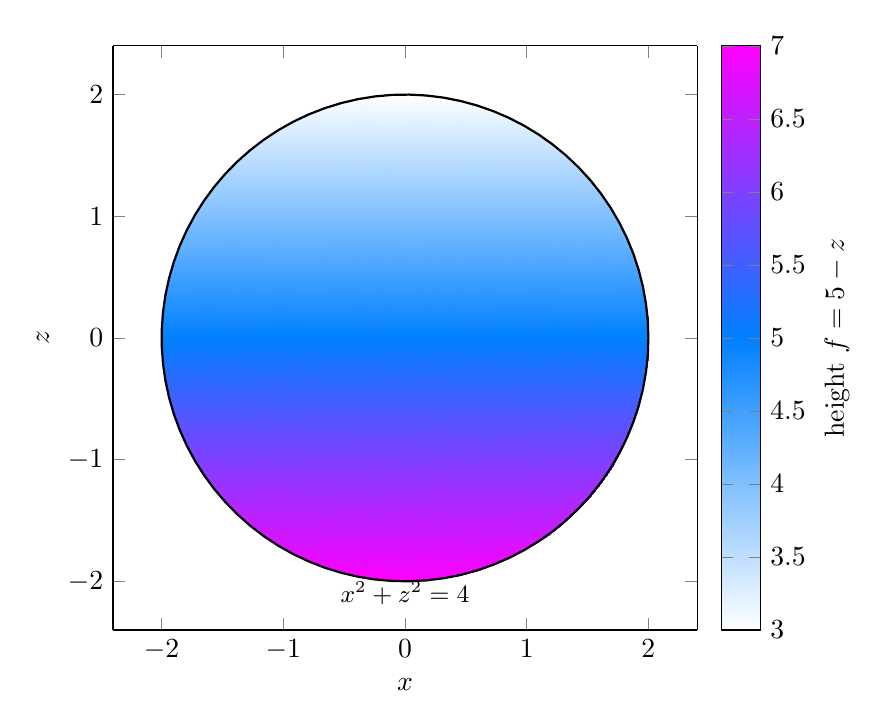
\begin{tikzpicture}
\begin{axis}[
  view={0}{90}, axis equal image, width=9cm, height=9cm,
  xlabel=$x$, ylabel=$z$,
  colormap/cool, colorbar,
  colorbar style={ylabel={height $f=5-z$}},
  xmin=-2.4, xmax=2.4, ymin=-2.4, ymax=2.4,
]
\addplot3[surf, shader=interp, domain=0:360, y domain=0:2, samples=80, samples y=16]
  ({y*cos(x)}, {y*sin(x)}, {5 - y*sin(x)});
\addplot3[domain=0:360, samples=90, thick, black, no markers]
  ({2*cos(x)}, {2*sin(x)}, {7});
\node at (axis cs:0,-2.1) {\small $x^2+z^2=4$};
\end{axis}
\end{tikzpicture}
\end{document}
